\documentclass[a4paper, 11pt, titlepage, english]{article}

\usepackage{babel}
\usepackage[latin1]{inputenc}
\usepackage[T1]{fontenc, url}
\usepackage{textcomp}
\usepackage{amsmath, amssymb}
\usepackage{amsbsy, amsfonts}
\usepackage{graphicx, color}
\usepackage{parskip}
\usepackage{framed}
\usepackage{amsmath}
\usepackage{xcolor}
\usepackage{multicol}
\usepackage{url}
\usepackage{flafter}
\usepackage{caption}
%\DeclareCaptionLabelSeparator{colon}{. }
\renewcommand{\captionfont}{\small\sffamily}
\renewcommand{\captionlabelfont}{\bf\sffamily}
\usepackage{float}
%\floatstyle{ruled}
%\restylefloat{figure}
\setlength{\captionmargin}{20pt}
%\addto\captionsenglish{\renewcommand{\figurename}{Fig.}}

\usepackage{geometry}
\geometry{headheight=0.01mm}
\geometry{top=24mm, bottom=30mm, left=39mm, right=39mm}






%
% Parametere for inkludering av kode fra fil
%
\usepackage{listings}
\lstset{language=python}
\lstset{basicstyle=\ttfamily\small}
\lstset{frame=single}
\lstset{keywordstyle=\color{red}\bfseries}
\lstset{commentstyle=\itshape\color{blue}}
\lstset{showspaces=false}
\lstset{showstringspaces=false}
\lstset{showtabs=false}
\lstset{breaklines}

%
% Definering av egne kommandoer og miljøer
%
\newcommand{\dd}[1]{\ \text{d}#1}
\newcommand{\f}[2]{\frac{#1}{#2}} 
\newcommand{\beq}{\begin{equation}}
\newcommand{\eeq}{\end{equation}}
\newcommand{\bra}[1]{\langle #1|}
\newcommand{\ket}[1]{|#1 \rangle}
\newcommand{\braket}[2]{\langle #1 | #2 \rangle}
\newcommand{\av}[1]{\left| #1 \right|}
\newcommand{\op}[1]{\widehat{#1}}
\newcommand{\braopket}[3]{\langle #1 | \op{#2} | #3 \rangle}
\newcommand{\ketbra}[2]{\ket{#1}\bra{#2}}
\newcommand{\pp}[1]{\frac{\partial}{\partial #1}}
\newcommand{\ppn}[1]{\frac{\partial^2}{\partial #1^2}}

\renewcommand{\arraystretch}{2}
\setlength{\tabcolsep}{10pt}
\makeatletter
\renewcommand*\env@matrix[1][*\c@MaxMatrixCols c]{%
  \hskip -\arraycolsep
  \let\@ifnextchar\new@ifnextchar
  \array{#1}}
\makeatother

%
% Navn og tittel
%
\author{Candidate number 6}
\title{Midterm Exam \\ FYS2160}


\begin{document}
\maketitle
\newpage\null\thispagestyle{empty}\newpage
\setcounter{page}{1} 

\section*{Problem 1}
For an ideal gas we have the relation
\beq
PV^\alpha = K; \quad \alpha = \frac{C-C_P}{C-C_V},
\label{eq:P_V}
\eeq
where $K$ is a constant.

\subsection*{a)}
We will derive general expressions for the work $W$, heat $Q$ and change in entropy $\Delta S$ for an ideal gas under \emph{quasistatic} conditions, i.e., that all volume changes occur slowly enough for the gas to continually equilibrate.

We will then discuss these expressions for the special cases of an \emph{isothermal}, an \emph{isobaric}, an \emph{adiabatic} and an \emph{isochoric} process.


\subsubsection*{Work, $W$}
For quasistaic compression, we know that the work is given by the integral\footnote{See {\it Schroeder\ } p.\ 22.}
$$W = - \int_{V_{\rm i}}^{V_{\rm f}} P(V){\rm\ d}V, \qquad {\rm (quasistatic)},$$
from eq.\ \ref{eq:P_V} we have an expression for $P(V)$, inserting it we find
$$W = - K\int_{V_{\rm i}}^{V_{\rm f}} \frac{1}{V^\alpha} {\rm\ d}V,$$
assuming $\alpha \neq 1$, the integration gives
\beq
W = -K\left[\frac{1}{\alpha-1} \frac{1}{V^{\alpha-1}} \right]_{V_{\rm i}}^{V_{\rm f}} = \frac{K}{\alpha-1} \left( \frac{1}{V_{\rm f}^{\alpha-1} - V_{\rm i}^{\alpha-1}} \right).
\eeq

\subsubsection*{Heat, $Q$}
The heat capacity $C$ of a system is defined as 
$$C \equiv \frac{Q}{\Delta T},$$
Multiplying by $\Delta T$, and substituting $\Delta T = T_{\rm f} - T_{\rm i}$ we get
\beq
Q = C \bigg( T_{\rm f} - T_{\rm i}\bigg) = C\Delta T.
\eeq

\subsubsection*{Change in entropy, $\Delta S$}
For a quasistatic process the infinitesimal change in entropy is given by\footnote{See {\it Schroeder\ } p.\ 112.}
$${\rm d}S = \frac{Q}{T}, \qquad {\rm (quasistatic)},$$
here the heat $Q$ is infinitesimal, but we avoid writing ``${\rm d}Q$'' to avoid confusion. We use the heat capacity $C$ to substitute 
$$C \equiv \frac{Q}{{\rm d}T} \quad \Rightarrow \quad Q = C {\rm\ d}T,$$
giving
$${\rm d}S = C \frac{{\rm d}T}{T}.$$
We now integrate the equation
$$\int_{S_{\rm i}}^{S_{\rm f}} {\rm d}S = C\int_{T_{\rm i}}^{T_{\rm f}} \frac{1}{T}{\rm\ d}T,$$
which gives
\beq
\Delta  S = C\ln\frac{T_f}{T_i}.
\eeq

\subsubsection*{Discussion of the expressions in special cases}

\begin{description}
\item[i)---isothermal process, $\Delta T = 0$] $ $ \\ For an isothermal process the ideal gas law gives
$$PV = NkT = {\rm constant}, \quad \Rightarrow \quad \alpha = 1.$$

In our derivation of the expression for the work $W$, we assumed that $\alpha \neq 1$, so we see the expression can't be used for an isothermal process.

The heat capacity $C$ is ill-defined in an isothermal process $\Delta T = 0$. Basically, any heat that is put into the system, will be cancelled by the mechanical work done---so $C \rightarrow \infty$. Our general expression of the heat then becomes
$$Q = C\bigg(T_{\rm f} - T_{\rm i}\bigg) = \infty \cdot 0,$$
which is undefined. So we can't use this expression for an isothermal process either.

For the expression for change in entropy we run into the same problem
$$\Delta S = C \ln \frac{T_{\rm f}}{T_{\rm i}} = C \ln 1 = \infty \cdot 0, $$
which is undefined.

\item[ii)---isobaric process, $\Delta P = 0$] $ $ \\ For an isobaric process the heat capacity $C$ is equal to the heat capacity at constant pressure $C_P$. From this we see that
$$\alpha = \frac{C-C_P}{C-C_V} = \frac{0}{C_P - C_V} = 0, \quad \Rightarrow \quad PV^\alpha = P = K.$$

Inserting this into our expression for the work gives
$$W = \frac{K}{-1}\left(\frac{1}{V_{\rm f}^{-1} - V_{\rm i}^{-1}}\right) = -P\bigg(V_{\rm f} - V_{\rm i}\bigg) = -P\Delta V.$$

The heat becomes
$$Q = C_P\bigg(T_{\rm f} - T_{\rm i}\bigg) = C_P \Delta T. $$

And the change in entropy
$$ \Delta S = C_P\ln\frac{T_{\rm f}}{T_{\rm i}}. $$

\item[iii)---adiabatic process, $Q = 0$] $ $ \\
For an adiabatic process the heat capacity goes to 0, as we are changing the temperature $\Delta T \neq 0$ of the  system without using heat $Q=0$, alpha becomes
$$\alpha = \frac{C- C_P}{C-C_V} = \frac{C_P}{C_V} = \frac{f + 2}{f} = \gamma.$$

The work becomes
$$W = -\frac{K}{\gamma - 1}\bigg( \frac{1}{V_{\rm f}^{\gamma-1}} - \frac{1}{V_{\rm i}^{\gamma - 1}}\bigg).$$

The expression for heat gives
$$Q = C\Delta T = 0\Delta T = 0,$$
which agrees with the definition of an adiabatic process.

The change in entropy becomes
$$\Delta S = C\ln \frac{T_{\rm f}}{T_{\rm i}} = 0\ln\frac{T_{\rm f}}{T_{\rm i}} = 0,$$
so we see there is no change in entropy in a quasistatic adiabatic process.

\item[iv)---isochoric process, $\Delta V = 0$] $ $ \\
Using that $V_{\rm f} = V_{\rm i}$, the expression for work becomes
$$W = -\frac{K}{\alpha}\bigg(\frac{1}{V_{\rm f}^\alpha-1} - \frac{1}{V_{\rm i}^\alpha-1}\bigg) = 0,$$
so when the volume of the gas does not change, the net work on the gas must be 0.

For an isochoric process the heat capacity $C$ is equal to the heat capacity at constant volume $C_V$, using this we find that the heat and change in entropy becomes
$$Q = C_V \Delta T, \qquad \Delta S = C_V \ln \frac{T_{\rm f}}{T_{\rm i}}.$$

\end{description}

\subsection*{b)}
We will now study a heat engine that uses a monatomic ideal gas of $N$ atoms as a working substance. The heat engine runs through a cyclical process where each cycle consists of four quasistatic subprocesses:

\begin{center}
\begin{tabular}{c l}
$1 \rightarrow 2$ & Adiabatic compression of the gas from $V_1$ to $V_2$,\\[-0.2cm]
$2 \rightarrow 3$ & Isochoric heating of the gas at volume $V_2$, \\[-0.2cm]
$3 \rightarrow 4$ & Adiabatic expansion of the gas from $V_2$ to $V_1$, \\[-0.2cm]
$4 \rightarrow 1$ & Isochoric cooling of the gas at volume $V_1$.
\end{tabular} 
\end{center}

We will illustrate this cycle in a pressure-volume diagram, and a entropy-volume diagram. We will also discuss the efficiency of the engine and analyze in what subprocesses the engine does work, absorbs heat $Q_h$ and expels heat $Q_c$.

\subsubsection*{Illustrating the cycle in a $PV$-diagram}
For the adiabatic compression and expansion, the ideal gas follow the expression
$PV^\gamma = {\rm constant},$
meaning these subprocesses can be illustrated as \emph{adiabats} in the $PV$-diagram. The subprocess $1\rightarrow 2$ is a compression, and so the adiabat will go towards lower volumes, and higher pressures. The subprocess $3\rightarrow 4$ is an expansion, so the adiabat will go to higher volumes and lower pressures. As adiabates connect isotherms, we know that the gas must increase in temperature with the compression, and decrease in temperature with the expansion.

For the isochoric heating and cooling of the gas the volume $V$ is constant at respectively $V_2$ and $V_1$. When the gas receives heat, the pressure $P$ will increase, and when the gas expels heat, the pressure $P$ will decrease.

\begin{figure}[htbp]
\centering
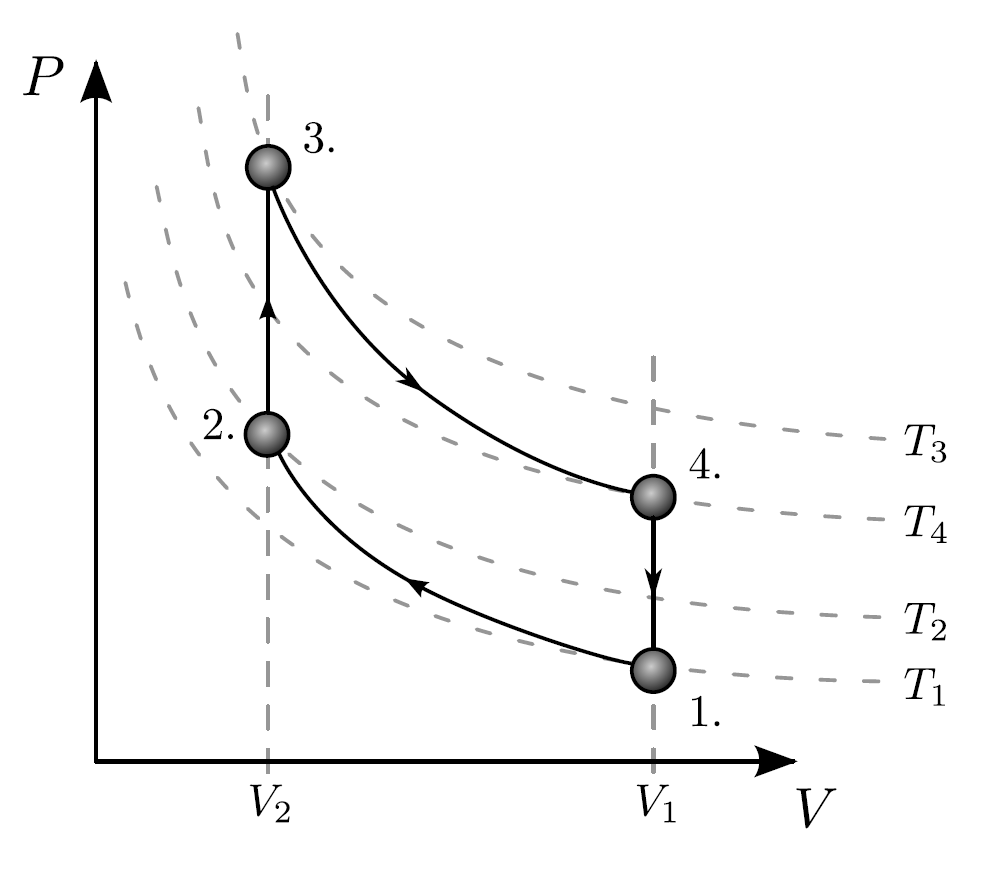
\includegraphics[width=0.6\textwidth]{PV}
\caption{An illustration of the heat engines cycle in a pressure-volume diagram. The curved and dotted lines represent isotherms. We see that the temperature in each point of the cycle is different: $T_3 > T_4 > T_2 > T_1.$ } \label{fig:PV}
\end{figure}

\clearpage


\subsubsection*{Illustrating the cycle in a SV-diagram}
We now have to analyze how the entropy $S$ changes in each subprocess. 

In problem 1a, we found that the change in entropy for a quasistatic adiabatic process is zero.
$$\Delta S = 0, \qquad {\rm (quasistatic,\ adiabatic)},$$
this means that the entropy is unchanged in the adiabatic subprocess $S_2 \rightarrow S_1$ and $S_4 \rightarrow S_3$.

In the isochoric subprocesses, the change in entropy will be given by
$$\Delta S = \frac{Q}{T}, \qquad {\rm (quasistatic)},$$
as the gas absorbs heat in subprocess $2 \rightarrow 3$, the entropy must increase, and as the gas expels heat in subprocess $4 \rightarrow 1$,  the entropy must decrease. For one complete cycle, the entropy of the engine must remain unaltered, so the entropy gained in $2\rightarrow3$ must be lost in $4\rightarrow1$.

We can now draw an illustration of the cycle in a $SV$-diagram
\begin{figure}[htbp]
\centering
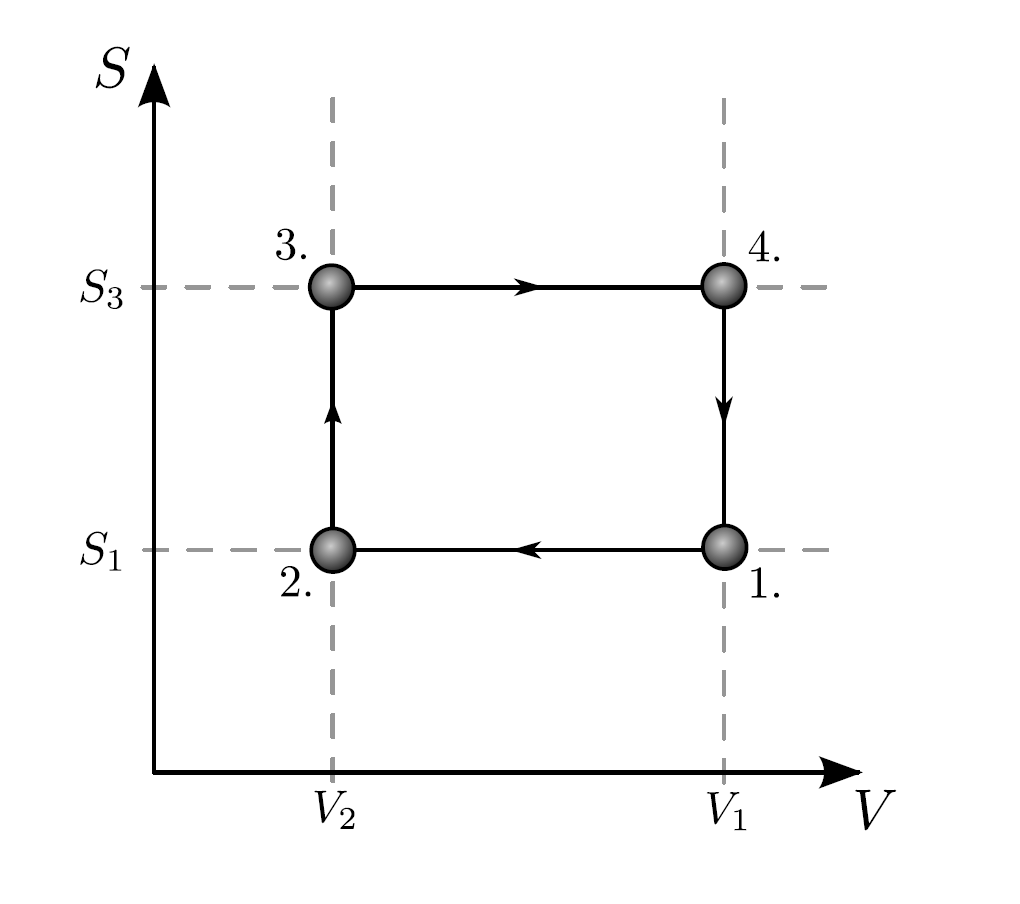
\includegraphics[width=0.6\textwidth]{SV}
\caption{An illustration of the heat engines cycle in a entropy-volume diagram.} \label{fig:SV}
\end{figure}

\subsubsection*{Analyzing the efficiency of the engine}

The efficiency of a heat engine is defined as the ratio between the {\it benefit} and the {\it cost}. In this case, the benefit is the net work performed by the engine on the environment, and the cost is the heat absorbed.
$$e \equiv  \frac{\rm benefit}{\rm cost} = \frac{W_{\rm net}}{Q_h}.$$
To get a better understanding of these quantities, we draw a black box illustration of the heat engine.

\begin{figure}[t]
\centering
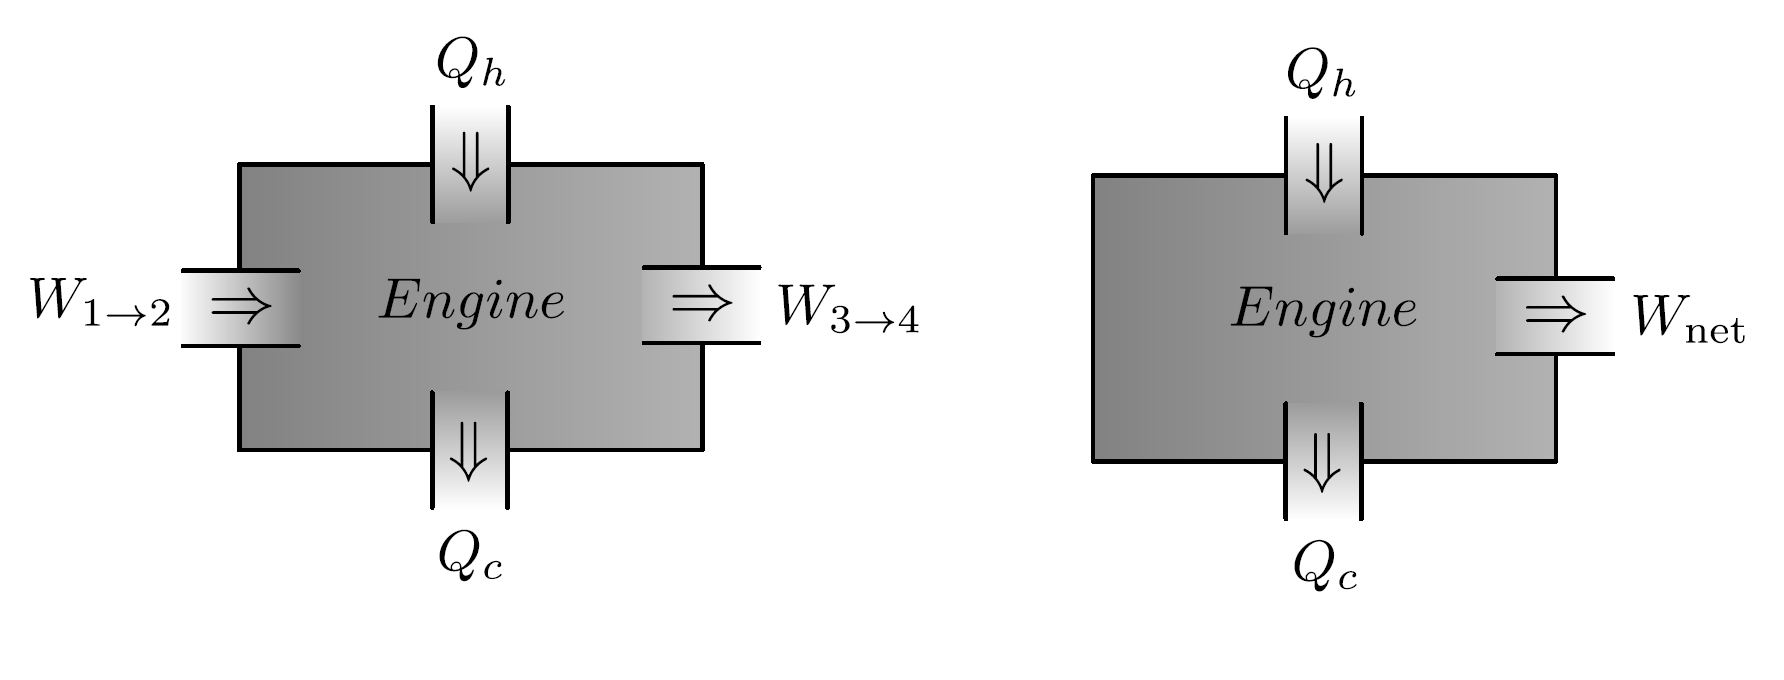
\includegraphics[width=\textwidth]{Engine}
\caption{An illustration of the heat engine as a black box, we are only concerned with the input and output of the engine, not the internal workings. On the left we view the work done on the gas as it is compressed as an input and the work done by the gas on the environment as an output---while on the right we simply view the net work performed by the engine on the environment as an output. \label{fig:blackbox}}
\end{figure}

From energy conservation, we know that the energy input of the machine must be equal to the energy output of the machine, so from figure \ref{fig:blackbox} and the fact that we have defined all quantities to be positive, we see that
$$W_{1\rightarrow2} + Q_h = W_{3\rightarrow4} + Q_c,$$
or simply
$$Q_h = W_{\rm net} + Q_c, \quad \Rightarrow \quad W_{\rm net} = Q_h - Q_c.$$
Inserting this expression for the net work into our expression for the efficiency of the engine gives us
$$e = \frac{Q_h - Q_c}{Q_h}.$$

\subsubsection*{Analyzing the work and heat}
From figure \ref{fig:PV}, \ref{fig:SV} and \ref{fig:blackbox} we see that the environment does work on the gas in subprocess $1\rightarrow2$ as the gas is compressed, we see that the gas absorbs heat $Q_h$ and entropy from the environment in subprocess $2\rightarrow3$ as it heats up, we see that the gas does work on the environment in subprocess $3\rightarrow4$ as it expands and we see that the gas expels heat $Q_c$ and entropy into the environment in subprocess $4\rightarrow1$. 

\subsection*{c)}
We will decide the heat $Q_h$ that the system receives in the $2\rightarrow 3$ subprocess and the heat $Q_c$ that the system expels in the $4\rightarrow1$ subprocess. 

These processes are isochoric and quasistatic, so we know that there is no work done,
$$\qquad \Delta U = Q, \qquad (\rm isochoric,\ quasistatic)$$ 
we can also express the change in energy from the equipartition principle 
$$Q = \Delta U = \frac{f}{2}Nk\Delta T = \frac{3}{2}Nk\Delta T,$$
where we have used that the gas has three degrees of freedom ($f=3$). We can express the difference in temperature as a difference in volumes and pressures using the ideal gas law
$$Nk\Delta T = NkT_{\rm f} - NkT_{\rm i} = P_{\rm f}V_{\rm f} - P_{\rm i}V_{\rm i},$$
the volume is constant in an isochoric processes, so
$$Q = \frac{3}{2}V(P_{\rm f} - P_{\rm i}).$$

To find $Q_h$ we only need to insert the right indices
$$Q_h = \frac{3}{2}V_2(P_3 - P_2),$$
To find $Q_c$ however, we must remember that $Q = -Q_c$ in the subprocess $4\rightarrow1$ as we have defined $Q_c$ to be positive, and the engine is expelling heat. This gives
\begin{align*}
Q_c &= -\frac{3}{2}V_1(P_1 - P_4) \\
&= \frac{3}{2}V_1(P_4 - P_1).
\end{align*}
Which is indeed positive, as $P_4 > P_1$ (see fig.\ \ref{eq:P_V}).

\subsection*{d)}
We will find the efficiency of the engine expressed solely by the ratio of the volumes $V_1$ and $V_2$, solely by the ratio of the temperatures $T_1$ and $T_2$ and solely by the ratio of the temperatures $T_4$ and $T_3$.

We start from the expression for the efficiency we found in problem 1b,
$$e = \frac{Q_h - Q_c}{Q_h}.$$
Inserting our expressions for $Q_h$ and $Q_c$ found in the previous problem gives
$$e = 1 - \frac{(3/2)V_1(P_4 - P_1)}{(3/2)V_2(P_3 - P_2)} = 1 - \frac{V_1}{V_2} \frac{P_4 - P_1}{P_3-P_2}.$$
We can find $P_3$ expressed by $P_4$ and $P_2$ expressed by $P_1$, the subprocesses $1\rightarrow2$ and $3\rightarrow4$ are adiabatic and in problem 1a we found that for an adiabatic
$$PV^\gamma = {\rm const.}, \qquad \gamma = \frac{f+2}{f} = \frac{5}{3}.$$
This means we can write
$$P_1V_1^{5/3} = P_2V_2^{5/3} \quad \Rightarrow \quad P_1 = \left(\frac{V_1}{V_2}\right)^{-5/3}P_2,$$
$$P_4V_4^{5/3} = P_3V_3^{5/3} \quad \Rightarrow \quad P_4 = \left(\frac{V_1}{V_2}\right)^{-5/3}P_3,$$
where we used $V_3 = V_2$ and $V_4 = V_1$. This means that we can rewrite
$$\frac{P_4 - P_1}{P_3 - P_2} = \left(\frac{V_1}{V_2}\right)^{-5/3},$$
and we can write the efficiency as
$$e = 1 - \left(\frac{V_1}{V_2}\right)^{-2/3} = 1 - \left(\frac{V_2}{V_1}\right)^{2/3}.$$

For a quasistatic and adiabatic process we know that\footnote{See {\it Schroeder } p.\ 25--26.}
$$ VT^{f/2} = {\rm const.} $$
For the adiabatic subprocess $1\rightarrow2$ we get
$$V_1T_1^{3/2} = V_2T_2^{3/2} \quad \Rightarrow \quad \left(\frac{V_2}{V_1}\right)^{2/3} = \frac{T_1}{T_2},$$
and for subprocess $3\rightarrow4$, using $V_3 = V_2$ and $V_4 = V_1$, we get
$$V_3T_3^{3/2} = V_4T_4^{3/2} \quad \Rightarrow \quad \left(\frac{V_2}{V_1}\right)^{2/3} = \frac{T_4}{T_3}.$$

So the efficiency can be written
$$e = 1 - \left(\frac{V_2}{V_1}\right)^{2/3} = 1 - \frac{T_1}{T_2} = 1 - \frac{T_4}{T_3}.$$

\subsection*{e)}
We will compare the efficiency of the heat engine with the efficiency of a Carnot-cycle. We will also analyze the change in entropy in both the engine and the reservoirs  for each subprocess and the cycle as a whole.

\subsubsection*{Efficiency}
The highest temperature the working gas in the engine reaches during a cycle is $T_h = T_3$ and the lowest temperature the working gases reaches during a cycle is $T_c = T_1$, see figure \ref{fig:PV}.

A Carnot-cycle can reach the efficiency,\footnote{See {\it Schroeder } p.\ 125.}
$$e_{\rm Carnot} = 1 - \frac{T_c}{T_h} = 1 - \frac{T_1}{T_3},$$
which is the maximum efficiency any heat engine can ever reach. The efficiency was in the last problem found to be
$$e = 1 - \frac{T_4}{T_3},$$
and as $T_4 > T_1$ we see that the efficiency for the heat engine is lower than that of the Carnot-cycle
$$e < e_{\rm Carnot}.$$

\subsubsection*{Change in entropy}
The sub processes $1\rightarrow2$ and $3\rightarrow4$ are adiabatic and so leads to no change in entropy in either the engine or the reservoirs.

In the subprocess $2\rightarrow3$ the hot reservoir is expelling heat and so loses entropy. As this process is quasistatic we can find the change in entropy from
$$\Delta S = \frac{Q}{T}, \qquad {(\rm quasistatic)}$$
the heat expelled is $Q = -Q_h$ and the temperature is $T_h$ throughout the process (we assume that the reservoir is so large that its temperature doesn't change even though it is expelling heat), so we find
$$\Delta S_{\rm R} = -\frac{Q_h}{T_h} = -\frac{3}{2}\frac{V_2}{T_3}(P_3-P_2) = -\frac{3}{2}\frac{V_2P_3}{T_3}(1 - \frac{P_2}{P_3}) = -\frac{3}{2}Nk(1 - \frac{P_2}{P_3}).$$
We cannot use the same expression for the change in entropy in the engine as the temperature, $T$, of the engine is changing throughout the process and is generally $T < T_3$, meaning the engine is gaining more entropy than the hot reservoir is losing. To find the change in entropy of the engine we use the result we found for an isochoric process in problem 1a
$$\Delta S_{\rm E} = C_V \ln \frac{T_{\rm f}}{T_{\rm i}} = \frac{3}{2}Nk \ln \frac{T_3}{T_2} = \frac{3}{2}Nk \ln \frac{P_3}{P_2},$$
where the ideal gas law was used to replace $T_3/T_2$ with $P_3/P_2$.

Similarly for the subprocess $4\rightarrow1$ we find the engine has a change in entropy
$$\Delta S_{\rm E} = \frac{3}{2}Nk \ln \frac{T_1}{T_4} = -\frac{3}{2}Nk \ln \frac{T_4}{T_1} = -\frac{3}{2}Nk \ln \frac{P_4}{P_1} = -\frac{3}{2}Nk \ln \frac{P_3}{P_2},$$
where we used that the ratios $P_3/P_2$ and $P_4/P_1$ are the same, this was shown in problem 1d. We see $\Delta S_{\rm E}$ is negative, which is good as the engine is expelling heat in this sub process. The cold reservoir is absorbing heat and so has an increase in entropy
$$\Delta S_{\rm R} = \frac{Q_c}{T_c} = \frac{3}{2}\frac{V_1}{T_1}(P_4 - P_1) = \frac{3}{2}Nk(\frac{P_4}{P_1} - 1) = \frac{3}{2}Nk(\frac{P_3}{P_2}-1).$$

We gather these results in a table, see table \ref{tabel:delta_s} on the next page. 

\subsubsection*{Discussion}
From the table we see that the entropy gained by the engine as a result of absorbing the heat $Q_h$ is lost when the engine expels the heat $Q_c$. Thus the change in entropy for the engine after one full cycle is $0$ as expected, remembering the SV-diagram. We also see however, that the cold reservoir has gained more entropy than the hot reservoir has lost, so the entropy of the environment has increased after one complete cycle. Thus the entropy of the engine and environment combined has increased, as expected from the second law of thermodynamics.

\begin{table}[p]
\centering
\begin{tabular}{|c|c|c|c|}
\hline			& $\Delta S_{\rm engine}$ & $\Delta S_{\rm reservoirs}$ & $\Delta S_{\rm total}$ \\[0.2cm] \hline
$1\rightarrow2$	& 0 & 0 & 0 \\[0.2cm] \hline
$2\rightarrow3$	& $\dfrac{3}{2}Nk\ln\dfrac{P_3}{P_2}$ & $-\dfrac{3}{2}Nk\left(1 - \dfrac{P_2}{P_3}\right)$ & $\dfrac{3}{2}Nk\left(\ln\dfrac{P_3}{P_2} - 1 + \dfrac{P_2}{P_3}\right)>0$  \\[0.2cm] \hline
$3\rightarrow4$	& 0 & 0 & 0  \\[0.2cm] \hline
$4\rightarrow1$	& $-\dfrac{3}{2}Nk\ln\dfrac{P_3}{P_2}$ & $\dfrac{3}{2}Nk\left(\dfrac{P_3}{P_2}-1\right)$ & $\dfrac{3}{2}Nk\left(\dfrac{P_3}{P_2} - 1 - \ln\dfrac{P_3}{P_2}\right)>0$  \\[0.2cm] \hline\hline
Full cycle		& 0 & $\dfrac{3}{2}Nk\left(\dfrac{(P_2-P_3)^2}{P_2P_3}\right)$ &  $\dfrac{3}{2}Nk\left(\dfrac{(P_2-P_3)^2}{P_2P_3}\right) > 0$ \\[0.2cm] \hline
\end{tabular}
\caption{The change of entropy in the engine, the change in entropy in the reservoirs combined and the total change in entropy for the system and the environment combined, for for each of the four subprocess and for one complete cycle.} \label{tabel:delta_s}
\end{table}

\cleardoublepage

\section*{Problem 2}
We will look at a monatomic ideal gas of $N$ atoms that occupies a two-dimensional area $A$ instead of a three dimensional volume $V$. The gas can only move in two dimensions, and thus has two degrees of freedom. It can be shown that multiplicity of the gas can me approximated as
$$\Omega(U,A,N) = \frac{1}{N!}\frac{A^N}{h^{2N}}\frac{\pi^N}{N!}(2mU)^N.$$

\subsection*{a)}
We will find an expression for the entropy of the gas as a function of the energy $U$, the area $A$ and the number of particles $N$.

We start from the definition of the entropy
$$S \equiv k \ln \Omega,$$
where $K$ is the Boltzmann constant. Inserting our expression for the multiplicity $\Omega$ gives,
\begin{align*}
S(U,A,N) &= k \ln \bigg[\frac{1}{N!}\frac{A^N}{h^{2N}}\frac{\pi^N}{N!}(2mU)^N\bigg] \\
&= k\bigg[N\ln U + N\ln A + N\ln\left(\frac{2\pi m}{h^2}\right) - 2\ln N!,\bigg]
\end{align*}
Using the coarser Stirling's approximation
$$\ln N! \approx N\ln N - N,$$
we find
\begin{align*}
S(U,A,N) &= k\bigg[N\ln A + N\ln U + N\ln\left(\frac{2\pi m}{h^2}\right) - 2N\ln N + 2N \bigg] \\
&= Nk\bigg[\ln U + \ln A   + \ln\left(\frac{2\pi m}{N^2 h^2}\right) + 2\bigg],
\end{align*}
we note that the last three terms in the bracket depend only on $N$ and so we introduce the shorthand notation
$$f(N) = \ln\left(\frac{2\pi m}{N^2 h^2}\right) + 2.$$
The entropy of the gas can then be written
$$S(U,A,N) = Nk\bigg[\ln U + \ln A + f(N)\bigg].$$

\subsection*{b)}
We will find the temperature $T$, the two-dimensional pressure-analogue $P$ (force per length), and the chemical potential $\mu$ for the gas.

\subsubsection*{Temperature, $T$}
The definition of temperature is 
$$\frac{1}{T} \equiv \left(\frac{\partial S}{\partial U}\right)_{N, A},$$
where the $N$ and $A$ subscript denotes that we hold the number of particles and the area of gas constant.

Inserting our expression for the entropy and treating $N$ and $A$ as constants gives
\begin{align*}
\frac{1}{T} &= Nk\bigg[\frac{\partial}{\partial U}\ln U + \frac{\partial}{\partial U} \ln A + \frac{\partial}{\partial U} f(N)\bigg] \\
&= \frac{Nk}{U},
\end{align*}
meaning the temperature of the gas is given by
$$T = \frac{U}{Nk}.$$

We see that the temperature is proportional to the energy $U$, inversely proportional to the number of particles $N$, and independent of the area $A$.

From the expression for the temprature we can derive an expression for the energy of the gas
$$T = \frac{U}{Nk} \quad \Rightarrow \quad U = NkT.$$
From the equipartition principle we find the alternate expression for the energy,
$$U = N\frac{f}{2}kT.$$
The gas has two degrees of freedom, so $f=2$ and the two expressions agree perfectly.

\subsubsection*{Pressure-analogue, $P$}
We can calculate the three-dimensional pressure (force per area) from the expression,
$$P = T\left(\frac{\partial S}{\partial V} \right)_{U,N},$$
so the two-dimensional analogue (force per length) can be found from
$$P = T\left(\frac{\partial S}{\partial A} \right)_{U,N}.$$
Inserting for the entropy and treating $N$ and $U$ as constants gives
\begin{align*}
P &= NkT\bigg[\frac{\partial }{\partial A}\ln U + \frac{\partial }{\partial A}\ln A + \frac{\partial }{\partial A}f(N) \bigg] \\
&= \frac{NkT}{A}.
\end{align*}

So the pressure-analogue of the gas is
$$P = \frac{NkT}{A} = \frac{U}{A}.$$

We see the pressure is proportional to the temperature $T$, inversely proportional to the area $A$ and independent of the number of particles $N$.

From the expression of the pressure we get
$$P = \frac{NkT}{A} \quad \Rightarrow \quad PA = NkT,$$
which is the two-dimensional equivalent of the ideal gas law:
$$PV = NkT.$$

\subsubsection*{Chemical potential, $\mu$}
The chemical potential is defined as
$$\mu \equiv -T\left(\frac{\partial S}{\partial N}\right)_{U,A}.$$
Inserting for the entropy and treating $U$ and $A$ as constants gives
\begin{align*}
\mu = -T\bigg[ \frac{\partial}{\partial N} Nk\ln U + \frac{\partial}{\partial N} Nk\ln A + \frac{\partial}{\partial N} Nk f(N)\bigg].
\end{align*}
Calculating the differentiation of $Nkf(N)$ separately using the product rule:
\begin{align*}
\frac{\partial}{\partial N} Nk f(N) &= kf(N) + Nk\frac{\partial}{\partial N}f(N) \\ 
&= kf(N) + Nk\frac{\partial}{\partial N}\left(\ln\left(\frac{2\pi m}{N^2 h^2}\right) + 2\right) \\
&= kf(N) - Nk\frac{N^2h^2}{2\pi m}\frac{4\pi m}{N^3h^2} \\
&= kf(N) - 2k \\
&= k\ln\left(\frac{2\pi m}{N^2 h^2}\right).
\end{align*}
Inserting this back in, we get
$$\mu = -kT\bigg[\ln U + \ln A + \ln\left(\frac{2\pi m}{N^2 h^2}\right)\bigg],$$
or written more compactly
$$\mu = -kT \ln \bigg[\frac{2\pi mUA}{N^2 h^2}\bigg].$$

We see that the chemical potential of the gas is a complicated function of all three variables: $U$, $A$ and $N$. The chemical potential of a three-dimensional ideal gas is
$$\mu = -kT \ln \bigg[\left(\frac{2\pi mkT}{h^2}\right)^{3/2}\frac{V}{N}\bigg], \qquad {\rm (3D,\ ideal\ gas)}$$
And we see that if we insert our expression for the energy of our two-dimensional gas ($U=NkT$), the chemical potential looks similar in the 2D-case only with $A$ instead of $V$ and missing the $3/2$-exponent due to $f/2$ being 1 instead of $3/2$.

\clearpage

\subsection*{c)}
The heat capacities of the gas at constant area $A$ and constant pressure $P$ are defined as
$$C_A \equiv \left( \frac{\partial U}{\partial T}\right)_{A,N}, \qquad C_P \equiv \left(\frac{\partial H}{\partial T}\right)_{P,N},$$
where $H$ is the enthalpy, which for a two-dimensional gas is defined as
$$H \equiv U + PA.$$
We will calculate these heat capacities for the ideal gas and use the thermodynamic identities to express these heat capacities as derivatives of the entropy.


\subsubsection*{Calculating $C_A$ and $C_P$}
From the definitions we find the heat capacities of the gas to be
$$C_A = \left( \frac{\partial U}{\partial T}\right)_{A,N} = \left( \frac{\partial }{\partial T} NkT\right)_{A,N} = Nk,$$
and
$$C_P = \left( \frac{\partial H}{\partial T} \right)_{P,N} = \left( \frac{\partial }{\partial T} (U + PA) \right)_{P,N} = \left( \frac{\partial H}{\partial T} 2NkT \right)_{P,N}  = 2Nk.$$
So we see that the heat capacities at constant area and pressure only depend on $N$, and that the heat capacity at constant pressure is always twice as large as the heat capacity at constant area.
For an ideal gas in three dimensions we know that\footnote{See {\it Schroeder\ } p.\ 30.}
$$C_P = C_V + Nk \quad {(\rm ideal\ gas)},$$
and we have now shown that the same relation holds for an ideal gas in two dimensions
$$C_P = C_A + Nk \quad {(\rm ideal\ gas)}.$$

\subsection*{Expressing $C_A$ and $C_P$ as derivatives of $S$}
The thermodynamic identities for $U$ and $H$ in two dimensions are
\begin{align}
dU &= TdS - PdA + \mu dN,\\
dH &= TdS + A dP + \mu dN.
\end{align}

Assuming the gas doesn't gain or lose particles $N$ is constant and $dN = 0$. From the first identity we then get
$$dU = T dS - P dA,$$
dividing by $dT$ and holding the area constant ($dA = 0$) we get
$$\left(\frac{\partial U}{\partial T}\right)_{A,N} = C_A = T \left(\frac{\partial S}{\partial T}\right)_{A,N}. $$

From the second identity we get
$$dH = T dS + A dP,$$
dividing by $dT$ and holding the pressure constant ($dP = 0$) we get
$$\left(\frac{\partial H}{\partial T}\right)_{P,N} = C_P = T \left(\frac{\partial S}{\partial T}\right)_{P,N}.$$

\subsection*{d)}
We will derive a Maxwell relation for a two-dimensional system.

The thermodynamic identity for Helmholtz free energy, which is defined as
$$F \equiv U - TS,$$
is in two-dimensions given as
$$dF = -S dT - PdA + \mu dN.$$

The mixed partial derivative of the Helmholtz free energy does not depend on which derivative is taken first so generally
\beq
\frac{\partial}{\partial A} \left( \frac{\partial F}{\partial T} \right) = \frac{\partial }{\partial T}\left(\frac{\partial F}{\partial A} \right). \label{eq:mixed}
\eeq
Where the area is held fixed when we take the partial derivative with respect to $T$ and vice versa. We will assume the number of particles $N$ to always be constant. 

We find from the thermodynamic identity for $F$
$$\left(\frac{\partial F}{\partial T}\right)_{A, N} = -S, \qquad \qquad \left(\frac{\partial F}{\partial A}\right)_{T, N} = -P.$$

Inserting these expressions back into equation \ref{eq:mixed} gives
$$\left(\frac{\partial S}{\partial A}\right)_{T,N} = \left(\frac{\partial P}{\partial T}\right)_{A, N},$$
this Maxwell relation holds generally for a two-dimensional system.

\subsection*{e)}
We will find an expression for the partial derivative of the entropy with respect to the temperature of the gas when the pressure and number of particles are held fixed,
$$\left( \frac{\partial S}{\partial T}\right)_{P,N}.$$

We start by looking at the entropy as a general function of temperature $T$, area $A$ and number of particles $N$. We can then express the differential $dS$ as
$$dS = \left(\frac{\partial S}{\partial T}\right)_{A, N} dT + \left(\frac{\partial S}{\partial A}\right)_{T, N} dA + \left(\frac{\partial S}{\partial N}\right)_{T, A} dN.$$
Assuming that the number of particles of the gas doesn't change, the last term becomes zero. We also see that the first term is equal to $C_A/T\ dT$ (see problem 2c). So $dS$ can be expressed as
\beq
dS = \frac{C_A}{T} dT +  \left(\frac{\partial S}{\partial A}\right)_{T, N} dA. \label{eq:dS}
\eeq

We will now look at the entropy instead as a general function of temperature $T$, pressure $P$ and number of particles $N$. We can do this as we have earlier shown that the pressure $P$ is a function of the temperature $T$, number of particles $N$ and area $A$. So any function that can be expressed by $T$, $A$ and $N$ can be expressed as $T$, $P$, and $N$. We can now write the differential $dS$ as
$$dS = \left(\frac{\partial S}{\partial T}\right)_{P, N} dT + \left(\frac{\partial S}{\partial P}\right)_{T, N} dP,$$
where we have skipped writing the term with $dN$ as it is zero when $N$ is constant. From this expression we get
$$\left( \frac{\partial S}{\partial T}\right)_{P,N} dT = dS - \left(\frac{\partial S}{\partial P}\right)_{T, N} dP.$$
Inserting equation \ref{eq:dS} for the differential $dS$ gives
\beq
\left( \frac{\partial S}{\partial T}\right)_{P,N}dT = \frac{C_A}{T}dT +  \left(\frac{\partial S}{\partial A}\right)_{T, N} dA - \left(\frac{\partial S}{\partial P}\right)_{T, N} dP. \label{eq:dA}
\eeq

We now look at the area as a general function of $T$, $P$ and $N$ and express the differential $dA$ as
$$dA = \left(\frac{\partial A}{\partial T}\right)_{P,N} dT + \left(\frac{\partial A}{\partial P}\right)_{T,N} dP,$$
where we again have used $dN = 0$. Inserting this expression for $dA$ in equation \ref{eq:dA} gives
\begin{align*}
\left( \frac{\partial S}{\partial T}\right)_{P,N}dT &= \frac{C_A}{T}dT -  \left(\frac{\partial S}{\partial P}\right)_{T, N} dP \\ &\qquad\qquad +  \left(\frac{\partial S}{\partial A}\right)_{T, N}\left[\left(\frac{\partial A}{\partial T}\right)_{P,N}dT + \left(\frac{\partial A}{\partial P}\right)_{T,N}dP\right]   \\[0.4cm]
&= \frac{C_A}{T}dT + \left(\frac{\partial S}{\partial A}\right)_{T, N}\left(\frac{\partial A}{\partial T}\right)_{P,N} dT \\ &\qquad\qquad + \left(\frac{\partial S}{\partial A}\right)_{T, N}\left(\frac{\partial A}{\partial P}\right)_{T,N}dP - \left(\frac{\partial S}{\partial P}\right)_{T, N} dP.
\end{align*}
As both derivations hold the same variables constant we can rewrite
$$\left(\frac{\partial S}{\partial A}\right)_{T, N}\left(\frac{\partial A}{\partial P}\right)_{T,N}dP = \left(\frac{\partial S}{\partial A}\frac{\partial A}{\partial P}\right)_{T,N}dP = \left(\frac{\partial S}{\partial P}\right)_{T,N} dP.$$
And we see the last two terms now cancel, leaving
\begin{align*}
\left( \frac{\partial S}{\partial T}\right)_{P,N} dT &=\frac{C_A}{T}dT + \left(\frac{\partial S}{\partial A}\right)_{T, N}\left(\frac{\partial A}{\partial T}\right)_{P,N} dT
\end{align*}
Using the Maxwell relation derived in the last problem
$$\left(\frac{\partial S}{\partial A}\right)_{T,N} = \left(\frac{\partial P}{\partial T}\right)_{A, N},$$
we find
$$ \left( \frac{\partial S}{\partial T}\right)_{P,N}dT = \frac{C_A}{T}dT + \left(\frac{\partial P}{\partial T}\right)_{A, N}\left(\frac{\partial A}{\partial T}\right)_{P,N} dT,$$
finally, dividing by $dT$ we find our final expression
$$ \left( \frac{\partial S}{\partial T}\right)_{P,N} = \frac{C_A}{T} + \left(\frac{\partial P}{\partial T}\right)_{A, N}\left(\frac{\partial A}{\partial T}\right)_{P,N}.$$

\end{document}
